\section{Design}

The design goals of NVKV are five-fold:
\begin{enumerate}
	\item \textbf{Direct Access}: BNVM should be operated on \textit{directly},
		without operating system interposition and without additional copies, as
		much as possible. This is possible in Linux using BNVM drivers and DAX
		\texttt{mmap}~\cite{dax}, wherein an application can memory map the
		actual BNVM directly into its address space.
	\item \textbf{Consistency with Operations}: Once each operation returns to
		the application, any changes required by the operation must be
		persistent. For example, after the insert function returns, the new data
		and the updated information in the index must be persisted to BNVM such
		that if power failed at that point, the insert operation would be safe.
	\item \textbf{Consistency with Power Failures}: NVKV must support power
		failures at \textit{any} point during \textit{any} operation. When power
		is resumed, and the application restarted, it should be able to continue
		operating without the database having been corrupted. In this case, we
		define free from corruption as all values that were inserted can be
		found, all items that were deleted cannot be found, all data that was in
		the database remains the same across power failures, and keys and values
		match as expected.

		If a power failure occurs in the middle of an insert, there is a
		possibility that the insert only partially completely. That is fine, as
		long as the above requirements are met. For example, the data might be
		copied in before the index is updated. If the power fails here, the only
		``inconsistency'' would be that there is a key-value pair that is not
		retrievable, which does not violate the above requirements because the
		insert operation had not yet returned to the user. However, this
		database state is sub-optimal since it contains unnecessary data. For
		these kinds up inconsistencies, we allow a fsck tool to be run to
		measure reachability for all keys and values and ensure that the
		database count is correct. Note that if the database was used without
		running the fsck tool, it would work as expected; the fsck tool is just
		there to optimize the database when power failures occur.
	\item \textbf{Performance}: Like any good key-value store, NVKV aims to
		provide the design requirements while being high performance.
		Specifically, it aims to be \textit{low-latency} to match the
		low-latency access to persistent storage that BNVM provides.
	\item \textbf{Compatibility}: To ease evaluation, NVKV provides an identical
		interface to Berkeley DB. When developing a new system, adoption is key,
		and backwards compatibility is vital for increasing adoption.
\end{enumerate}

The design choices in NVKV fit some common themes. The first theme is to make
each update to the database that is done by an operation like insert a series of
small, consistent sub-operations. Each of these sub-operations moves the
database from one valid state to another, possibly with the use of a transaction
(which, to avoid confusion, in this document means ``a transaction using
transactional memory on some memory``). The database is carefully designed to
allow it to \textit{always} construct each operation out of a bounded number of
sub-operations that keep the database in a consistent state. The second common
theme is to avoid data movement as much as possible. While this is not always
possible when rehashing, NVKV bounds the number of moved words on \textit{every}
insert.

One significant reason we strive for these goals is that we are designing a
system using a transactional memory primitive that does not exist yet. However,
we can expect that such a system will operate somewhat like a transaction: a
\texttt{transaction-begin}, followed by a bounded number of instructions,
followed by \texttt{transaction-commit} or \texttt{abort}. We expect the number
of instructions and the number of memory accesses allowed inside the transaction
to be bounded, at least due to the performance costs of having large
transactions, but at most because the hardware support might directly limit it.
Thus, we are designing pessimistically; should transactional memory support
exceed our expectations, NVKV will still work, however we can reasonably assume
that it will fit within the requirements of most reasonable transactional memory
proposals. The assumption is that both number of instructions and number of
memory accesses matter, although the number of memory accesses is more
important.

\subsection{Interface}

The interface to applications provided by NVKV is just like Berkeley DB. In
fact, the only difference is in the header file that must be included by the
application (\texttt{db.h} in the case of \bdb and \texttt{nvkv.h} in the case
of NVKV). Applications then link with \texttt{libnvkv.so}. The interfaces are
exactly the same, although a lot of functionality is left unimplemented, as full
compatibility is well outside the scope of a class project. The implemented
functionality is \texttt{db\_create}, \texttt{db\_open}, \texttt{get},
\texttt{put}, \texttt{sync}, \texttt{err}, \texttt{errx}, and manipulation of
\texttt{DBT}s. The format of the database files is \textit{not} compatible; only
the programming interface is.

\subsection{Data Organization}

The database file contains two separate types of data: data and metadata. Data
refers to the contents of a \texttt{DBT} (keys and values) along with their
lengths. The exact format of the data storage is discussed in
section~\ref{sec:ds}. Metadata is the information kept by the database in order
to support the lookup operations on the data; that is, a small structure
containing information about the database as a whole, and the indexing data
structure.

\begin{figure}
\centering
\hspace*{-0.1in}
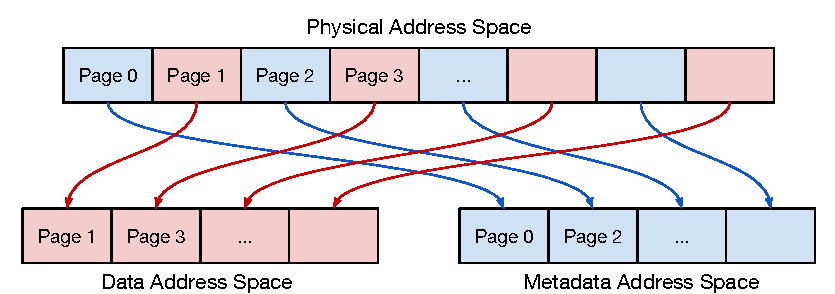
\includegraphics[width=84mm]{fig/addrspace}
\caption{Mapping the data and metadata address spaces to the physical address
space of the database file.}
\label{fig:addrspace}
\end{figure}

Since NVKV maintains backwards compatibility with \bdb, it is allowed only one file to
store both metadata and data. However, both of these grow when inserting,
meaning that if they were placed naively inside the database file, they might
have to be moved. Moving large amounts of data is fine in a database system
such as \bdb, but when operating directly on BNVM, we must avoid moving data
when possible. Furthermore, moving data is much more difficult to do in a single
transaction.

To avoid moving data, NVKV lays out memory as shown in
figure~\ref{fig:addrspace}, where each page of metadata is interlaced with each
data page. Logically, this provides two separate, linear address spaces for data
and metadata. Internal pointers are stored \textit{as if} these address spaces
were real and started at zero; that is, if page-size is 4K and we wished to
write a pointer to the second page of metadata, it would be \texttt{0x1000 +
page-offset}, even though the actual location in the file this refers to is
\texttt{0x2000 + page-offset}. When swizzling pointers into their virtual
address space value after \texttt{mmap}ing the database, NVKV relies on context
to choose the address space, apply the appropriate operation to determine the
offset into the file, and then adds the base address of the \texttt{mmap}
region to calculate the ultimate virtual address.

The need to deal with persistent pointers in virtual memory is a real problem,
because we can no longer have an explicit serialization step when persisting to
persistent memory---after all, the data is already persistent. Thus, we must
always write pointers to memory in a universal format that applications can make
use of regardless of the ultimately mapped location of the data that is pointed
to or the pointers themselves. We are working on a larger project named
Twizzler~\cite{bittman-ssrctr-17-01} that addresses and explores these issues in
detail and provides a programming model based around transparent use of
universal pointers. If that system was fully functional, most of the complexity in this
key-value store would be trivial, since most of the code complexity comes from
dealing with swizzling between these different address spaces (data, metadata,
persistent, and virtual).


\subsection{Indexing}

The indexing structure we are using is a hash table, exploiting the
random-access and non-block-oriented nature of BNVM~\cite{Debnath:2016ht}. To
deal with collisions, we have chosen Cuckoo hashing~\cite{Pagh:2004}, a hashing
scheme that results in good cache locality, bounded lookups, and reasonably high
load-factor. Each key is hashed to two buckets, $b_1 = H_1(k) \mod l$ and $b_2 =
H_2(k) \mod l$, where $k$ is the key, $l$ is the table length, and $H_1$ and
$H_2$ are two different hash functions. When inserting, bucket $b_1$ is
evaluated, and if it is empty, the key is inserted there. If it is not empty, we
look at $b_2$. If \textit{it} is empty, we can insert there. Otherwise, we must
\textit{move} the contents of either $b_1$ or $b_2$ before we can insert. This
process is shown in figure~\ref{fig:insert}, where $B$ must move for $A$ to be
inserted.

\begin{figure}
\centering
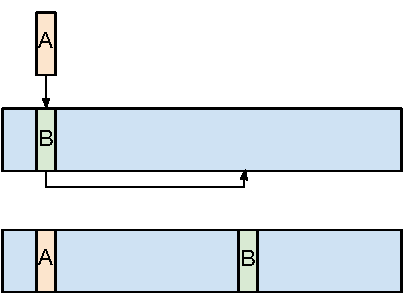
\includegraphics[width=70mm,height=50mm]{fig/cuckoo_insert}
\caption{Inserting an element that requires moving an existing element to a
partner bucket.}
\label{fig:insert}
\end{figure}


To move $B$, we determine its partner bucket (the other bucket it hashes to),
and try to move it there. If there is an item in the partner bucket, we
recursively try to move until we are successful. Note that cycles are possible;
should a cycle occur (or a threshold number of moves is reached), the move is
aborted and a rehash is triggered. When inserting, if both $b_1$ and $b_2$ are
full, and neither can be moved, the hash table is rehashed---the length is
doubled.

Lookup is implemented by checking both $b_1$ and $b_2$ for the key. This is a
strength of Cuckoo hashing, that lookup operations take a bounded, small number
of steps while still supporting collision resolution.

\paragraph{Rehashing}

Rehashing is the most arduous part of dealing with hash tables, for it often
involves a large pause and a significant amount of data movement. Reinserting
all the keys into a double-length table is not viable for NVKV, because we are
trying desperately to avoid excessive data movement and because it is difficult
to define this in terms of a bounded transaction. A possible solution would be
to pass off the reinsertions into future insert operations, but that can get
complicated should a rehash be triggered a second time shortly thereafter.
Furthermore, this increases the complexity of insert operations.

Instead, NVKV takes the approach of just not reinserting the data. The table
length is still doubled, causing new inserts to be distributed throughout the
new table, but old data still remains clustered in the first half, untouched, as
shown in figure~\ref{fig:rehash}.
The lookup operation is modified to try looking up for each size the hash table
has been; that is, it calculates $b_1 = H_1(k) \mod l$ (and $b_2$ similarly),
followed by $b_1 = H_1(k) \mod \frac{l}{2}$, and so on, until it reaches the
original size of the hash table. We are essentially treating the table as a set
of tables, each twice the size of the previous, overlapping in memory.

We always insert ``at the top level'', meaning that inserts and moves are always
done with the current value of $l$ and no other. When a collision is found, it
is moved to its partner bucket (calculated with $l$) even if it was originally
there from a previous value of $l$. Although the data from a previous $l$ is
clustered in the first half of the table ($l$ was just doubled; the second half
is empty), it is unlikely to cause a large number of movements immediately
because new inserts have equal likelihood to end up in the second half of the
table. Next, when an old value must move, it has equal likelihood of being moved
to the second half of the table, thereby eventually spreading the data out
across the table. The advantage of this is no extra code complexity; the data is
eventually spread through the normal operation of inserts and moves.


\begin{figure}
\centering
\hspace*{1mm}
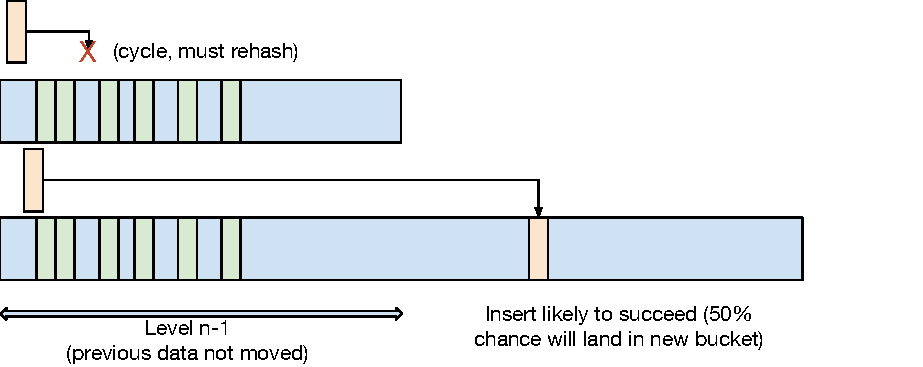
\includegraphics[width=90mm]{fig/cuckoo_rehash}
\caption{Extending the hash table to level $n$ without reinserting existing
elements. Level $n-1$ has existing elements that are not moved during the
expansion, and the newly inserted element is more than twice as likely to find
an empty bucket to insert into.}
\label{fig:rehash}
\end{figure}

The end result is a hash table that does not require expensive rehashing while
providing bounded insert operations at the expense of slightly slower lookup
operations. However, we found that although lookups have to try looking up
assuming several different values of $l$, in practice the data was redistributed
quite quickly, causing most insert operations to only lookup one level.


\paragraph{Why Cuckoo?}

Cuckoo hashing dove-tails nicely with the rehashing scheme. One of the reasons
this scheme would not work with something like linear probing is that lookups in
linear probing are not bounded. Looking up at each ``level'' (value of $l$) must
be bounded and fast for the additional requirement to lookup at each level to be
reasonable. Linear probing would end up searching a large number of buckets for
each lookup, which is infeasible. Cuckoo hashing limits the bucket search at
each level to two.
Another advantage is that Cuckoo hashing already does data movement as part of
its implementation, meaning that the clustered data after a rehash will be
automatically spread out. 


For BNVM and transactional memory, we must both limit the size of the
sub-operations and make each one leave the index in a consistent state. Movement
in Cuckoo hashing achieves both goals; each movement requires only a small
number of memory operations onces the system decides to move a bucket somewhere,
and each one remains consistent. If a key were to move from $b_1$ to $b_2$, it
will still be locatable because it \textit{could have} been in $b_2$ all along.
The lookup will still find it. This properly allows the recursive move function
to move data in these sub-operations, always with the index consistent. Even if
the recursion gets interrupted part-way through and power is lost, the database
will remain valid.




\subsection{Data Storage}
\label{sec:ds}

Data storage of keys and values is currently implemented much like an arena
allocator; an ``end'' pointer is kept and incremented whenever a new \texttt{DBT} is
recorded. Recording a \texttt{DBT} involves copying the data into the data
address space along with its length. The address of the copied-in length and
data is calculated, after which it can be used to refer to the data internally.
The end pointer is incremented by the data length plus the size of the length
field, allowing the next \texttt{DBT} to be written directly after it. Note
that, because of the address space interleaving described above, adding data to
the database never causes it to interfere with the metadata.

To ensure persistence and consistency, the end pointer is not updated until
after the data is copied in. After each word of data copied, the cache-line
is flushed and a memory fence is applied, ensuring that the data be flushed back
to BNVM. A potential optimization could be to only flush when crossing a
cache-line boundary. The reason we do not use a transaction here is that the
data could be arbitrarily long. Once the data is copied, the end pointer is
incremented and flushed. Again, a transaction is not needed here because we are
only updating a single value.




